% =============================================================================
%  Section 1 -- Problem & Motivation
% =============================================================================

\section{Problem \& Motivation}

% --- Section divider -----------------------------------------------------------
\sectiondivider{Problem \& Motivation}{Why paddle tennis players need data-driven feedback}

% --- The Sport & Access Gap ----------------------------------------------------
\begin{frame}{Paddle Tennis: a growing sport with limited feedback tools}
\begin{columns}[T,onlytextwidth]
\begin{column}{0.56\textwidth}
\begin{itemize}
    \item Padel is one of the fastest-growing racket sports (Europe, Latin America).
    \item Played mostly in doubles on an enclosed court with playable glass walls.
    \item \alert{Amateurs} rely on self-evaluation or sporadic coach feedback.
\end{itemize}
\vspace{6pt}
\begin{block}{Access barriers for amateurs}
\begin{itemize}
    \item \kv{Lesson cost}{30--50~USD/session (CO/MX)}.
    \item \kv{Min.\ monthly wage}{$\sim$300--320~USD}.
    \item \kv{Video tracking}{$<$ 1 in 6 courts in MTY/Cali offer any motion analysis.}
\end{itemize}
\end{block}
\end{column}
\begin{column}{0.42\textwidth}
\centering
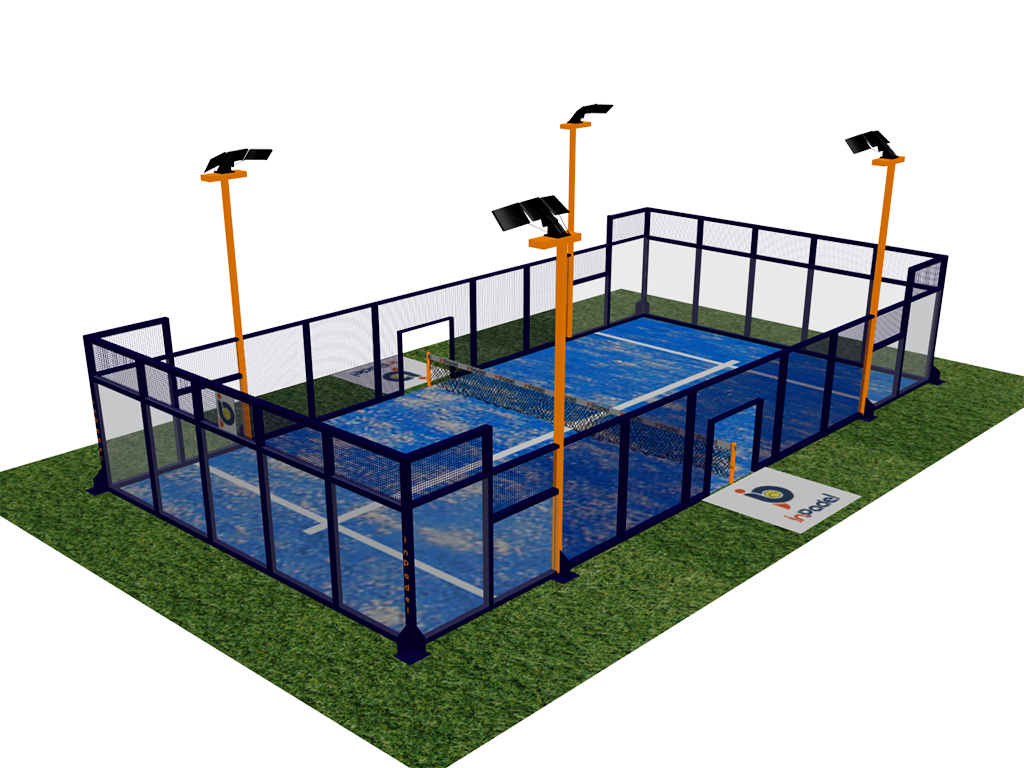
\includegraphics[width=\linewidth]{./DATA/images/intro/PaddleTennis_Court.png}\\
{\scriptsize\itshape Standard paddle tennis court with glass walls.}
\end{column}
\end{columns}
\end{frame}

% --- The Bandeja shot ----------------------------------------------------------
\begin{frame}{Why the \emph{bandeja} shot?}
\begin{columns}[T,onlytextwidth]
\begin{column}{0.55\textwidth}
\begin{itemize}
    \item Defensive overhead shot used to maintain net control after a lob.
    \item Biomechanically rich: arm extension, wrist position, impact timing, footwork.
    \item Mastery is what \alert{separates intermediate from advanced} amateurs.
    \item Ideal first target for an automated quality-assessment system.
\end{itemize}
\vspace{6pt}
\begin{exampleblock}{Scope of this thesis}
A single shot (\emph{bandeja}), a single output (5-class quality score), one reproducible end-to-end pipeline.
\end{exampleblock}
\end{column}
\begin{column}{0.43\textwidth}
\centering
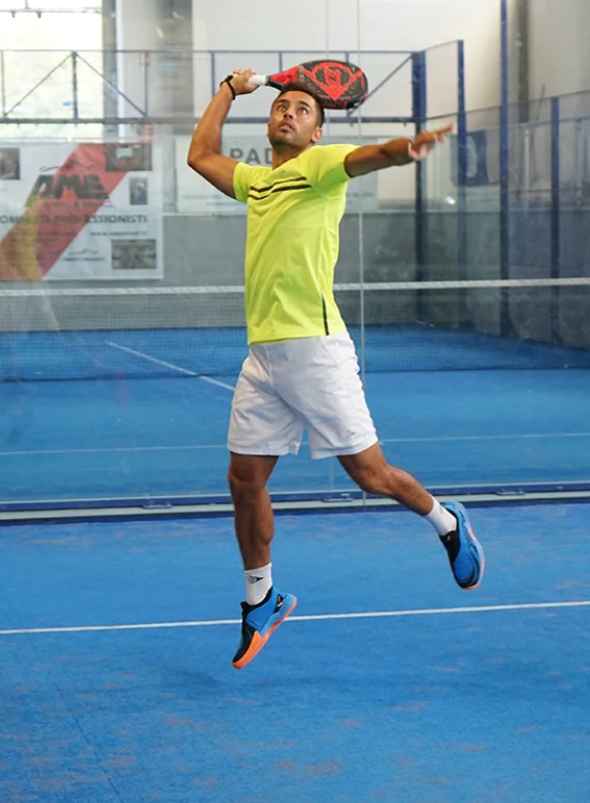
\includegraphics[width=0.95\linewidth]{./DATA/images/intro/Bandeja.png}\\
{\scriptsize\itshape The bandeja shot.}
\end{column}
\end{columns}
\end{frame}

% --- Hypothesis & Research Questions ------------------------------------------
\begin{frame}{Hypothesis \& Research Questions}
\begin{block}{Hypothesis}
\small A supervised \alert{recurrent model}, trained on pose-estimation data from \emph{bandeja} videos, can assign quality scores that are \alert{consistent with expert assessments} under controlled conditions.
\end{block}
\vspace{4pt}
\textbf{\color{tecdark}Research Questions:}
\begin{enumerate}\small
    \item How accurately does pose estimation extract key joints across skill levels?
    \item How well does the LSTM replicate expert-assigned scores, and with what deviation?
    \item To what extent does the model generalize to unseen performances?
    \item Is the learned representation specific to the \emph{bandeja}, or extensible to other shots?
\end{enumerate}
\end{frame}

% --- Contributions ------------------------------------------------------------
\begin{frame}{Contributions}
\begin{enumerate}\small
    \item A novel \alert{pose-based dataset} for paddle tennis: 484 \emph{bandeja} clips from 6 players, expert-graded (1--10) and mapped to 5 quality classes.
    \item Comparative evaluation of three temporal models -- \alert{BiLSTM, BiGRU, TCN} -- under identical pipeline, dataset, and metrics.
    \item Two sensitivity analyses (loss/optimizer grid and 5-point split sweep) that quantify how the system reacts to design choices.
    \item A fully \alert{reproducible end-to-end pipeline} (video $\rightarrow$ pose $\rightarrow$ sequence $\rightarrow$ classification) released as open-source code.
    \item Public release of the labeled dataset (2D joint trajectories + grades + metadata) as a benchmark for racket-sport motion analysis.
\end{enumerate}
\vspace{2pt}
\begin{infoBox}\small
Code: \url{https://github.com/CesarEmilioC/thesisRepo_A00830006}
\end{infoBox}
\end{frame}
